\begin{exercise}
		Να προσδιοριστούν:
	\begin{enumerate}
	  \item ο πίνακας $R_{\theta, y}$ και
	  \item ο πίνακας $R_{\theta, x}$.
	\end{enumerate}
\end{exercise}

\begin{solution}
\begin{enumerate}
	
\item  Επιλέγω αρχικά σημείο που να ανήκει στο Επίπεδο $xz$.
	
		Από το σχήμα προκύπτει ότι: 
		\begin{align*}
		x' &= x\cos{\theta} + z\sin{\theta}	\\
		y' &= y \\
		z' &= -x\sin{\theta} + z\cos{\theta}	
		\end{align*}
		
		Συνεπώς:
		
		\[
		R_{\theta, y}= 
		\begin{bmatrix}
		\cos{\theta} & 0 & \sin{\theta} & 0 \\
		0 & 1 & 0 & 0 \\
		-\sin{\theta} & 0 & \cos{\theta} & 0 \\
		0 & 0 & 0 & 1
		\end{bmatrix} 
		\]	
		
		\begin{figure}[hbt]
		\begin{center}
		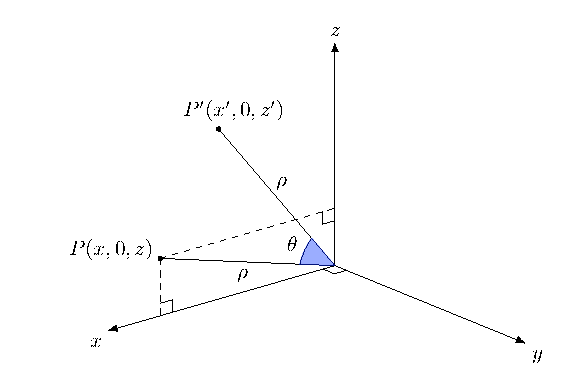
\includegraphics[scale=1]{Chapter3/point-in-xz-rotation.pdf}
		\end{center}
		\caption{Στροφή σημείου στο επίπεδο $xz$}
		\end{figure}

	
\item  Επιλέγω αρχικά σημείο που να ανήκει στο Επίπεδο $yz$.
	
		Από το σχήμα προκύπτει ότι: 
		\begin{align*}
		x' &= x \\
		y' &= y\cos{\theta} - z\sin{\theta}	\\
		z' &= y\sin{\theta} + z\cos{\theta}	
		\end{align*}
		
		Συνεπώς:
		
		\[
		R_{\theta, y}= 
		\begin{bmatrix}
		1 & 0 & 0 & 0 \\
		0 & \cos{\theta} & -\sin{\theta} & 0 \\
		0 & \sin{\theta} & \cos{\theta} & 0 \\
		0 & 0 & 0 & 1
		\end{bmatrix} 
		\]	
		
		\begin{figure}[hbt]
		\begin{center}
		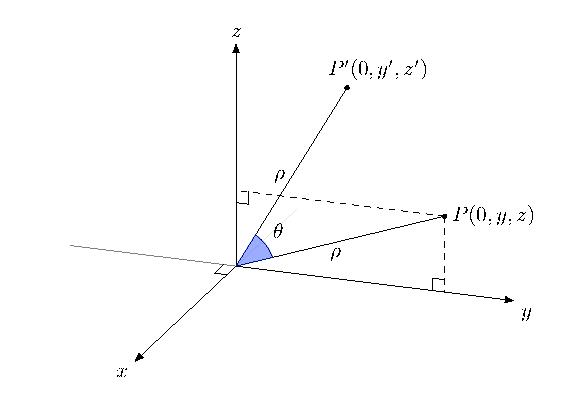
\includegraphics[scale=1]{Chapter3/point-in-yz-rotation.pdf}
		\end{center}
		\caption{Στροφή σημείου στο επίπεδο $xz$}
		\end{figure}
		
\end{enumerate}		
\end{solution}